\chapter{Annotated poem, \AS{كِسْوَاحِلِ} (\textit{Kiswahili}), 12pt, footnotes}
\renewcommand{\thesection}{D/\arabic{section}}  % redefine the section numbering
\setcounter{section}{0}  % reset counter 
\label{appD}

\citet{Abdulkadir2013} presents an annotated edition of the poem \AS{كِسْوَاحِلِ} by Mahmoud Ahmad Abdulkadir (Ustadh Mau).

The following is a letter-for-letter transcription of the author's manuscript as reproduced there, with the exception that the damma-with-tail occasionally used by him to signify \textbf{o} is denoted here with inverted damma (eg in \AS{كُوَأٗنَ نَ تَمَانِ} in 1d), since the font does not yet include that glyph.  The layout also includes an automatically-generated close transliterations, a standard transliteration based on that in the paper, and the English translation and notes from the paper.  The notes also include citations, with the references printed at the end of the document.

The document was generated automatically from a database table which held all the data about the poem (words, translation, notes, etc) -- see \Cref{ch:poetry}, and the \textit{kiswahili} table in the \url{andika/db/starter/andika} database included in the \textbf{Andika!} download.

The font-size is 12pt, and notes appear as footnotes.  For comparison, the same poem is printed in \Cref{appF} in a font-size of 10pt, with notes appearing as endnotes.

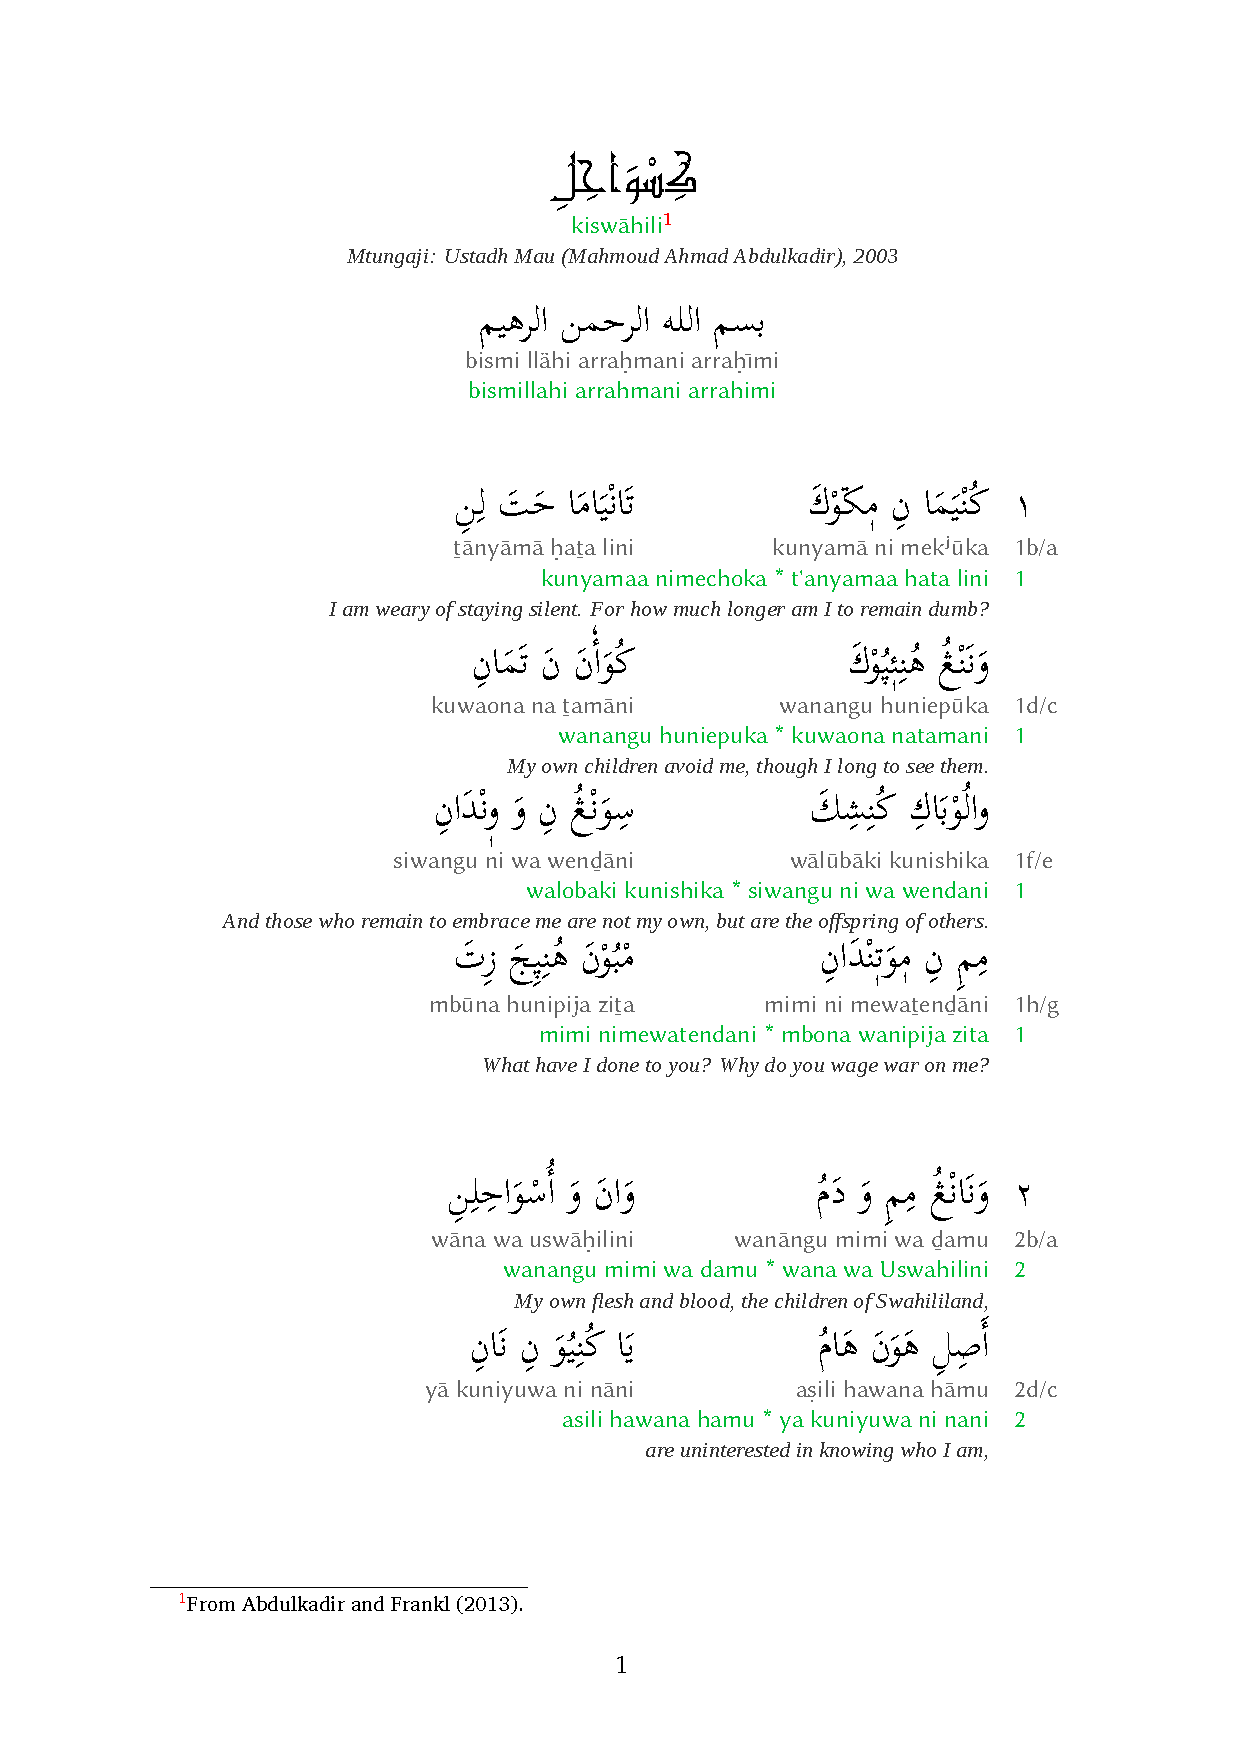
\includepdf[pages={ - }, pagecommand={}]{../db/outputs/kiswahili/kiswahili12pt-footnotes.pdf}

